\documentclass[11pt,a4paper]{article}
\usepackage[margin=2.2cm]{geometry}
\usepackage{fontspec}
\setmainfont{TeX Gyre Pagella}
\setmonofont{DejaVu Sans Mono}[Scale=0.82]
\usepackage{amsmath,amssymb,amsthm}
\usepackage{graphicx,xcolor,listings,booktabs,enumitem}
\usepackage[most]{tcolorbox}
\usepackage{tikz}
\usepackage{needspace}
\usepackage[hidelinks]{hyperref}

\definecolor{accent}{HTML}{2B6CB0}
\definecolor{warn}{HTML}{C53030}
\newtcolorbox{keybox}[1][]{colback=accent!5,colframe=accent,boxrule=0.6pt,arc=2pt,left=6pt,right=6pt,top=4pt,bottom=4pt,#1}
\newtcolorbox{warnbox}{colback=warn!5,colframe=warn,boxrule=0.6pt,arc=2pt,left=6pt,right=6pt}

\lstdefinelanguage{Rust}{
  keywords={fn,let,mut,if,else,for,in,while,return,use,pub,struct,impl,loop,break,Some,None,as,match,const,Self,self},
  morekeywords=[2]{usize,i32,i64,u64,f64,bool,Vec,VecDeque,BTreeSet,BTreeMap,BinaryHeap,Option,str},
  sensitive=true, morecomment=[l]{//}, morestring=[b]"}
\lstset{language=Rust,basicstyle=\ttfamily,keywordstyle=\color{accent}\bfseries,
  keywordstyle=[2]\color{teal},commentstyle=\color{gray}\itshape,stringstyle=\color{warn},
  frame=single,rulecolor=\color{gray!40},backgroundcolor=\color{gray!4},
  numbers=left,numberstyle=\tiny\color{gray},xleftmargin=1.5em,breaklines=true,
  columns=fullflexible,keepspaces=true,showstringspaces=false}

\newtheorem*{invariant}{Invariant}
\theoremstyle{definition}\newtheorem*{definition}{Definition}

\usepackage{soul}
\definecolor{hlY}{HTML}{FFF3A0}\definecolor{hlG}{HTML}{C8F2C2}\definecolor{hlP}{HTML}{E6D2F7}\definecolor{hlB}{HTML}{CFE3FF}
\newcommand{\hly}[1]{{\sethlcolor{hlY}\hl{#1}}}
\newcommand{\hlg}[1]{{\sethlcolor{hlG}\hl{#1}}}
\newcommand{\hlp}[1]{{\sethlcolor{hlP}\hl{#1}}}
\newcommand{\hlb}[1]{{\sethlcolor{hlB}\hl{#1}}}
\newcommand{\img}[3]{\begin{center}\fcolorbox{gray!50}{white}{\includegraphics[width=#1]{board/#2}}\\[-2pt]{\footnotesize\textcolor{gray}{#3}}\end{center}}
\newcommand{\extra}{\textsuperscript{\textcolor{warn}{[extra]}}}
% pages of the prof's 2025 notes on the Fenwick tree (Lessons/L11/FenwickTree_2025.pdf)
\newcommand{\oldnotes}[2]{\begin{center}\fcolorbox{gray!50}{white}{\includegraphics[page=#1,width=#2,trim=20 20 20 20,clip]{../L11/FenwickTree_2025.pdf}}\\[-2pt]
  {\footnotesize\textcolor{gray}{Prof.'s notes of \textbf{last year} (2025), \texttt{FenwickTree\_2025.pdf} p.\,#1}}\end{center}}
\newcommand{\twonotes}[2]{\begin{center}\begin{minipage}{0.49\textwidth}\centering\fcolorbox{gray!50}{white}{\includegraphics[page=#1,width=0.95\linewidth,trim=20 20 20 20,clip]{../L11/FenwickTree_2025.pdf}}\end{minipage}\hfill
  \begin{minipage}{0.49\textwidth}\centering\fcolorbox{gray!50}{white}{\includegraphics[page=#2,width=0.95\linewidth,trim=20 20 20 20,clip]{../L11/FenwickTree_2025.pdf}}\end{minipage}\\[2pt]
  {\footnotesize\textcolor{gray}{Prof.'s notes of \textbf{last year} (2025), \texttt{FenwickTree\_2025.pdf} p.\,#1 and p.\,#2}}\end{center}}
\newcommand{\board}[3]{\img{#1}{#2}{Board, #3 (recording \texttt{L\_12.MP4})}}
\title{\textbf{CPC --- Lecture 12}\\[2pt]\large Counting inversions with a Fenwick tree $\cdot$ Remapping $\cdot$ Nested Segments}
\author{Competitive Programming and Contests --- Monday 26/10/2026}
\date{}

\begin{document}\sloppy
\maketitle
\vspace{-1.5em}
\begin{keybox}
\textbf{Sources.} Recording \texttt{Lessons/L12/L\_12.MP4} (91 min) and its automatic transcript \texttt{L12\_transcript.txt} (not revised);
the prof's handwritten board (frames of the recording, \texttt{board/l12\_*.jpg});
the prof's 2025 notes \texttt{Lessons/L11/FenwickTree\_2025.pdf} (p.\,7--10 on today's topics);
the prof's blog post \emph{Dynamic Prefix Sums with Fenwick Tree} (\url{https://pages.di.unipi.it/rossano/blog/2023/fenwick}), code copied verbatim.
No notes of yours for this lecture. Everything marked \extra{} was \emph{not} said or written in the lecture (my explanations, examples, code).

\hlp{This replaces the provisional version of 27/10}, which had guessed the content from the 2025 notes. The guess was half right:
inversions with a Fenwick tree and Nested Segments \hlg{were done}, but with a \hlb{different solution of Nested Segments} (the one derived in class, \S\ref{sec:nested});
\hlp{Update the Array and range updates were not done}: they were explained on 28/10, see \texttt{Lessons/L13/L13.pdf}.

\smallskip
\noindent Code: \texttt{Lessons/L12/src} (\texttt{cargo test -p l12}). Exercises: \texttt{Lessons/L12/practice}, E50--E52 (\texttt{cargo test -p practice\_l12}).

\smallskip
\noindent\textbf{Highlights:} \hly{general / to remember} \quad \hlg{good: works, efficient, correct} \quad \hlp{bad: pitfalls, wrong ideas, costs} \quad \hlb{definitions and key results}
\end{keybox}

\begin{keybox}[colback=gray!4,colframe=gray!60]
\textbf{Where we are.} L11 (21/10) ended with counting inversions via mergesort and the question ``can we get the same running time using the Fenwick tree?''.
Today: the answer (0:00--14:00), the \textbf{remapping} trick and when it is worth it (14:00--40:00), then \textbf{Nested Segments}, solved together step by step (40:00--88:00).
\end{keybox}

\tableofcontents

%==========================================================
\section{Counting inversions with a Fenwick tree}
%==========================================================
\textbf{Recap.} Count the pairs $i<j$ with $A[i]>A[j]$, $A[1,n]$ of positive numbers $\le n$. The number of inversions is quadratic in the worst case,
and it is the number of steps of insertion sort. Mergesort variant (L11): every time the current minimum comes from the \emph{right}, add the number of
elements remaining on the \emph{left}: \hlg{\mbox{$\Theta(n\log n)$}}.

\noindent\textbf{Idea} (4:40--11:40). \hly{Process the array from left to right.} When we reach an element we want to know \hlb{how many elements to its left are greater}.
Keep an array $F$ with the \hlb{frequency of every value} (values in $1..6$), stored in a Fenwick tree.
The prof extends the example to $A=[3,2,1,6,5,4,3,2]$ (8 positions, values up to 6) ``to make clear that the frequency is the frequency of the \emph{value}, not of the position''.
\begin{itemize}[nosep]
\item ``On my left'': guaranteed because \hly{we update the frequencies while moving from left to right}, so only elements on my left are in $F$.
\item ``Greater than me'': the frequencies to the right of my value in $F$: a \hlb{suffix sum}, i.e.\ $\textsf{RangeSum}(A[i]+1,\ \mathrm{end})$ (``$+1$ because I don't want to count my value'').
\end{itemize}
\begin{lstlisting}[language={},numbers=none]
for i in range(len(A)):
    result += RangeSum(A[i] + 1, end)
    Add(A[i], 1)
\end{lstlisting}
\board{0.5\textwidth}{l12_fenwick_inversions.jpg}{14:40}
\textbf{Running time.} $n$ iterations, each a range sum and an add: $n\log(\max A)$. \hly{Another cost may become dominant}: initializing $F$, which has one position per possible value.
So \hlb{\mbox{$\Theta(\max(A)+n\log\max(A))$}} and, \hlg{if \mbox{$\max(A)\in O(n)$}, \mbox{$\Theta(n\log n)$}}. \extra{} With 8 elements the example has 14 inversions.
\needspace{12\baselineskip}\noindent\textbf{Prof's code} [blog] (verbatim; \texttt{l12::inversions::counting\_inversions}):
\begin{lstlisting}
pub fn counting_inversions(a: &[u64]) -> usize {
    if a.is_empty() {
        return 0;
    }

    let max = *a.iter().max().unwrap() as usize;
    let mut ft = FenwickTree::with_len(max + 1);

    let mut count: usize = 0;
    for &e in a {
        count += ft.range_sum((e + 1) as usize, max) as usize;
        ft.add(e as usize, 1);
    }

    count
}
\end{lstlisting}
\noindent\extra{} For $e=\max$ the call is \texttt{range\_sum(max + 1, max)} $=\textsf{sum}(\max)-\textsf{sum}(\max)=0$: fine. Tested against an $O(n^2)$ brute force and the mergesort version
on random arrays with duplicates and zeros.


%==========================================================
\section{Remapping the values}
%==========================================================
\hlp{If \mbox{$\max(A)$} is too big, \mbox{$F$} is too large}: with $A=[1,\,150,\,10^6,\,155,\,6,\,8]$ we pay $10^6$ just to initialize the tree, then 6 elements in the loop.
\begin{itemize}
\item It is similar to \hly{direct-access table vs hash map}: a direct-access table only when the maximum value is bounded and small, otherwise a hash map
      (and, as discussed before, \hly{always check whether a direct-access table is enough}).
\item A student suggests a hash map instead of $F$. \hlp{It solves only part of the problem}: it stores frequencies, but we need \emph{cumulative} frequencies over a range,
      computed efficiently, which is what the Fenwick tree gives. Use the map instead to \hlb{map each value to a position} in $1..n$ (at most $n$ distinct values), and build the Fenwick tree on $1..n$.
\item \textbf{Which mapping?} First attempt: a hash map and a counter, assigning ids in order of first appearance: $1\to1$, $150\to2$, $10^6\to3$, $155\to4$, $6\to5$, $8\to6$.
      \hlp{Wrong: it does not preserve the relative order of the values}, so the range sum ``after my value'' no longer contains the larger values
      (the elements greater than $10^6$ are not those mapped to $4..6$). ``There are many cases in which this makes a lot of sense, but not in this case.''
\item \hlb{Correct remapping: sort, then replace each value with its rank in the sorted order}: $1,6,8,150,155,10^6\ \to\ 1..6$, so $A$ becomes $[1,4,6,5,2,3]$.
\end{itemize}
\board{0.55\textwidth}{l12_remap.jpg}{39:40: the values, their ranks after sorting, and $\max(A)\in O(n^c)$}
\hlb{This and many other problems are insensitive to the actual values: the answer depends only on the relative order}, so remapping does not change it.
``\hly{From now on, if the values are too large, the first step is to remap them into a smaller range}.''

\subsection{Practical remarks}
\begin{itemize}[nosep]
\item Remapping with hash maps (value $\to$ rank) or with binary search on the sorted array (a student's suggestion): a technical choice.
      \hlp{Hash maps can be very expensive in practice}, ``pathologically slow in C''\,\footnote{\extra{} He presumably means C++'s \texttt{std::unordered\_map}.}; faster in Rust.
      \hly{Sorting is usually better than hash maps here} (locality, deterministic). \hlb{The only way to know which option is best for your case and language is to benchmark them}
      (``you usually have two or three options, test all of them''). Remapping happens a lot, not only in competitions.
\item Mergesort and duplicates: no problem, when two equal values are compared during the merge, just do not count them as an inversion.
\end{itemize}

\subsection{Is remapping + Fenwick tree worth it, compared to mergesort?}
A student's question: if we must sort anyway to remap, mergesort already sorts \emph{and} counts. The prof's answer:
\begin{itemize}
\item \textbf{In practice}: we don't know. Nobody uses mergesort in practice, but quicksort (asymptotically worse, faster in practice); a super-optimized quicksort followed by the
      Fenwick tree may beat a hand-written mergesort.
\item \textbf{Asymptotically}, it depends on the values.
  \begin{itemize}[nosep]
  \item \hlp{Unbounded values}: the remapping needs a comparison-based sort, $\Theta(n\log n)$ like mergesort, plus the Fenwick tree: \hlp{not better than mergesort}.
  \item \hly{Bounded values, \mbox{$\max(A)\in O(n^c)$} with \mbox{$c$} constant} (e.g.\ $n=1000$ values up to $10^6$ or $10^9$): \hlg{radix sort sorts in linear time}
        (that is exactly the bound of radix sort). Still, the Fenwick tree costs $n\log n$: \hlp{not better} either.
  \end{itemize}
  The mergesort solution is already ``more than satisfactory''; having two solutions with the same running time is not an issue.
\item \textbf{Why spend so much time on it?} \hlb{The remapping trick is worth in many other problems where there is no easy sorting-based solution.}
\end{itemize}
\noindent\extra{} \texttt{l12::inversions::remap} sorts the pairs (value, position), as in the 2025 notes (equal values get increasing ranks, still no inversion between them);
\texttt{counting\_inversions\_any} = remap + prof's code. Exercise E51 uses dense ranks (equal values, equal rank): both are correct.
\twonotes{7}{8}

%==========================================================
\section{Nested Segments (Codeforces 652D)}\label{sec:nested}
%==========================================================
\textbf{Problem.} We are given $n$ segments $\langle l_1,r_1\rangle,\dots,\langle l_n,r_n\rangle$ (all endpoints distinct).
\hlb{Report, for each segment, the number of segments it (fully) contains.}
Target: \hlg{\mbox{$\Theta(n\log n)$}}: with a Fenwick tree this means \hly{a range sum and possibly an add for each segment}.
\hly{First step: remap the segments' extremes, if needed} (numbering them $1..2n$).
\board{0.5\textwidth}{l12_nested_statement.jpg}{45:40: for the grey segment, the green ones are contained, the red one is not}

\noindent Running example on the board (already remapped): $[1,5],\ [2,10],\ [3,4],\ [6,8],\ [7,11],\ [9,12]$.
\extra{} Answers: $[1,5]\to1$, $[2,10]\to2$, all the others $0$. (The 2025 board had $[7,12],[9,11]$ instead.)

\subsection{The way to the solution (a discussion in class)}
\begin{enumerate}
\item \textbf{Two Fenwick trees}, $FT_{\text{start}}$ with a 1 at every beginning and $FT_{\text{end}}$ with a 1 at every end (a student). For $[2,10]$ the segments starting inside are
      $RangeSum$ on $FT_{\text{start}}$ over $(2,10]$: $3,6,7,9$, i.e.\ 4. \hlp{An overestimation}: $[7,11]$ and $[9,12]$ start inside but end after.
      Fixing it with $FT_{\text{end}}$ does not work: \hlp{the 1s of the two trees are not related to each other} (an end inside the segment may belong to a segment starting before).
      Counterexample: a segment with many segments starting inside and many ending inside, but none contained: the answer is 0.
\item \emph{Side remark.} The easier question ``how many segments \emph{intersect} me?'' is $n$ minus those that start after my end and those that end before my start:
      \hlg{static prefix sums are enough}, no Fenwick tree.
\item \textbf{Relate the two extremes} (another student): label every 1 in $FT_{\text{start}}$ with the end of its segment ($1\to5$, $2\to10$, $3\to4$, $6\to8$, $7\to11$, $9\to12$).
      Then the answer for $[2,10]$ is \hlb{the number of 1s in \mbox{$[2,10]$} whose label is smaller than 10} (minus myself): 2. \hlp{But no data structure answers
      ``how many values in this range are smaller than \mbox{$x$}'' efficiently.}
      (Compacting the labels into an array $[5,10,4,8,11,12]$ maps a range of starts to a subarray, but does not answer the query.)
\end{enumerate}
\board{0.6\textwidth}{l12_two_fenwick.jpg}{61:00: $FT_{\text{start}}$ and $FT_{\text{end}}$; the range of $[2,10]$ (red) over-counts}
\noindent\textbf{Two things we were not exploiting.}
\begin{itemize}[nosep]
\item \hlb{We are free to process the segments in any order we want} (we were answering each segment independently).
\item \hlb{The Fenwick tree can remove 1s} (``we were using the Fenwick tree without using its capabilities'': static prefix sums would have been enough).
\end{itemize}
``\emph{If you are writing your letter to Santa Claus}'': for $[2,10]$ I would ask to \hly{remove the 1s of the segments that end after 10}; then the 1s in $[2,10]$ are me plus
segments starting inside and, thanks to Santa Claus, ending before 10.
\board{0.55\textwidth}{l12_labels.jpg}{78:20: the 1s of $FT_{\text{start}}$ labelled with the end of their segment}

\subsection{The solution: decreasing end, remove after use}
``Let's implement Santa Claus'': \hlb{process the segments in decreasing order of ending point}. When we reach the segment ending at 10, the segments ending at 12 and 11 have already
been processed, and \hlb{each of them removed its own 1 from the Fenwick tree before leaving}.
\begin{lstlisting}[language={},numbers=none]
FT = 1 at the start of every segment            // after remapping the 2n extremes to 1..2n
for each segment [l, r] in decreasing order of r:
    answer[l, r] = RangeSum(l, r) - 1            // -1: my own start
    Add(l, -1)                                   // remove my 1 before leaving
\end{lstlisting}
Example: $[9,12]$: $RangeSum(9,12)=1$, answer $0$, remove 9. $[7,11]$: $1-1=0$ (\hlp{without removing 9 it would be 2}, wrong), remove 7.
$[2,10]$: $RangeSum(2,10)=3$ (2, 3, 6), \hlg{answer 2}, the correct one: the two segments that start inside but end after 10 were already removed.
(Or remove before the range sum, then no $-1$.) \hlg{One Fenwick tree, \mbox{$\Theta(n\log n)$}}, ``derived almost together''.
\board{0.55\textwidth}{l12_nested_solution.jpg}{83:00: ends circled, processed right to left; the 1s at 7 and 9 already set to 0 when $[2,10]$ is processed}

\noindent\textbf{Three versions of the problem} (a student's question, 83:30--87:30):
\begin{enumerate}[nosep]
\item this one: the segments are known, report the answer for each of them;
\item \hlp{online}: build a data structure; given \emph{any} segment, return how many segments it contains: \hlp{much harder};
\item \hly{offline queries}: a set of segments and a set of query segments, known in advance, so they can be reordered: \hlg{easier}, as in a previous lecture
      (Ilya and Queries, L9). The Fenwick tree is built on the segments only; process segments and queries together by decreasing end point:
      for a query do only the range sum, for a segment only the update. The prof was ``thinking about the solution while saying this'' and invited questions by message.
      \extra{} Details to fix if you implement it: a query does not subtract 1 (it is not in the tree), and ties between the end point of a query and of a segment need care.
\end{enumerate}

\noindent\textbf{Code.} No code from the prof. \extra{} \texttt{l12::nested::nested\_segments\_2026} is the lecture's solution;
\texttt{nested\_segments\_2025} (2025 notes p.\,10: increasing ends, \emph{insert} the starts) and \texttt{nested\_segments} (blog: increasing starts, Fenwick tree on the ends) are
the two equivalent alternatives; all tested on the board example, the Codeforces examples and against an $O(n^2)$ brute force.
\hly{On the course page it is the mandatory exercise of the 21/10/2026 row: try it yourself first (E52).} See \S\ref{sec:ex}.
\twonotes{9}{10}

\begin{keybox}
\textbf{About the pace (88:00).} The prof is going about twice as slowly as last year because he spends more time \hlb{deriving the solutions together} instead of
giving five minutes and then presenting his solution; he thinks it is better, ``especially in a time in which it's easy to get a solution almost for free''.
If you disagree, tell him (also anonymously). ``We need another lecture about this kind of stuff'': last year two lectures, this year three.
\end{keybox}

%==========================================================
\section{Exercises and deadlines (course page)}\label{sec:ex}
%==========================================================
\begin{keybox}
\textbf{For this lecture (26/10): nothing.} The 2026 table of the course page has \hlb{no row for 26/10} (checked on 29/10), and no homework was given orally.

\smallskip
\textbf{Still open, from earlier rows of this year's table} (2026, not last year's):
\begin{itemize}[nosep]
\item \textbf{Nested Segments}, \url{http://codeforces.com/problemset/problem/652/D}: mandatory in the row of \textbf{21/10/2026}. The technique was explained only today
      (the prof is slower than the plan of the page), so now you can solve it: practice E52.
\item \emph{Pashmak and Parmida's problem}, \url{http://codeforces.com/problemset/problem/459/D}: optional, row of 21/10/2026.
\item \textbf{Update the Array}, \url{http://www.spoj.com/problems/UPDATEIT/}: mandatory in the row of \textbf{19/10/2026}; explained on 28/10 (\texttt{L13.pdf}, practice E53).
\end{itemize}
\hly{The rows of the page are the prof's plan, not what happened in class}: the 21/10 row (``Applications of Fenwick tree and Range update'') is being covered on 26/10 and later.
\end{keybox}

%==========================================================
\section{Next time}
L13 (28/10, \texttt{Lessons/L13/L13.pdf}): Update the Array, dynamic prefix sums with range update (two Fenwick trees), introduction to the segment tree.

\end{document}
